
% Desc: Stage user manual
% Author: Richard Vaughan, Andrew Howard
% Date: 10 Jun 2002
% CVS: $Id: stage.tex,v 1.16 2002-06-11 08:29:57 rtv Exp $

\documentclass[11pt,twoside]{report}

% this one apparently fixes the < and > chars
\usepackage[T1]{fontenc}
\usepackage{subfigure}
\usepackage{times}
\usepackage{tabularx}

% why did we need this?
%\usepackage{verbatim}
% make all captions small and slanted
\usepackage[small,sl]{caption}
\usepackage{fullpage}
%\usepackage{epsf}
\usepackage{epsfig}
\usepackage{graphicx}
% add nifty DRAFT watermark thingy in PS
%\usepackage{draftcopy}

% A nice environment for displaying command line args (AH)
\newenvironment{xarg}[1]{\noindent{\tt #1}\\\hspace*{2em}\begin{minipage}[t]{5in}}{\end{minipage}\vspace*{1em}}

\def\VERSION {1.2}
\def\HOMEPAGE {{\tt http://playerstage.sourceforge.net}}
\def\SFPAGE {{\tt http://sourceforge.net/projects/playerstage/}}

\begin{document}

\setcounter{page}{0}
\pagenumbering{roman}

\titlepage

 \begin{tabular}{lcr}
   \begin{tabular}{c}
 	Player/Stage project\\
         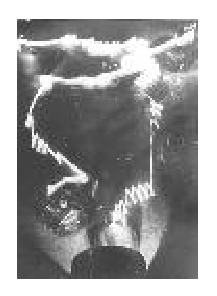
\includegraphics{notext_ps_logo}
    \end{tabular}
   &
   \hspace{5cm}
   &
   \begin{tabular}{r}
     {\bf USC Robotics Laboratory}\\
     University of Southern California\\
     Los Angeles, California, USA\\
     \vspace*{2em}\\
     {\bf Information Sciences Laboratory}\\
     HRL Laboratories\\
     Malibu, California, USA\\
   \end{tabular}
 \end{tabular}


  \vspace{5cm}	
  \centerline{ \Huge{Stage}}
  \vspace{0.5cm}
  \centerline{\large{Version \VERSION\ User Manual}}
  \vspace{2cm}
  \centerline{\large Richard T.~Vaughan \\ Andrew Howard \\ Brian P.~Gerkey}
  \vspace{1cm}

  \centerline{This document may not contain the most current documentation on}
  \centerline{Stage.  For the latest documentation, consult the Player/Stage homepage:}
  \centerline{\HOMEPAGE}

  \vspace{4cm}

 \centerline{\today}

\tableofcontents
%\newpage

%\listoffigures
%\newpage
%\listoftables
%\newpage

% reset page number to start with 1
\setcounter{page}{0}
\pagenumbering{arabic}


\chapter{Introduction}

  \section{What is Stage?}

    Stage simulates a population of mobile robots, sensors and objects
    in a two-dimensional bitmapped environment. Stage is designed to
    support research into multi-agent autonomous systems, so it
    provides fairly simple, computationally cheap models of lots of
    devices rather than attempting to emulate any device with great
    fidelity. We have found this to be a useful approach.

    Stage devices are usually controlled through \emph{Player}; a
    networked robot server. Player comes with a collection of device
    drivers for interfacing with real robots and sensors. Stage
    provides populations of virtual devices for Player. Users write
    robot controllers and sensor algorithms as 'clients' to the Player
    'server'. Typically, clients cannot tell the difference between
    the real robot devices and their simulated Stage equivalents
    (unless they try very hard). We have found that clients developed
    using Stage will work with little or no modification with the real
    robots and vice versa. Thus Stage allows rapid prototyping of
    controllers destined for real robots. Stage also allows
    experiments with realistic robot devices you don't happen to have.
  
    Various sensors and actuators are provided, including sonar,
    scanning laser rangefinders, vision (color blob detection),
    odometry, and a differential steer robot base.

  \section{How to get Stage and related software}

    The primary source for all things Player and Stage is the project
    homepage:\\\\ \indent \HOMEPAGE\\	
	
   \noindent Access to source code releases, access to the CVS
   development tree, bug tracking, user mailing lists, etc.~ is
   available from the Sourceforge project management page:\\\\\indent
   \SFPAGE\\

   \noindent The current release is available as the source tarball
 Stage-<version>.src.tgz at:\\\\ \indent
 http://sourceforge.net/project/showfiles.php?group\_id=42445\\

	Previous versions were significantly different; this manual
   does not apply to them.

  \section{What's in the Package?}

    In the release tarball you will find:
      \begin{itemize}    
      \item C++ source code for 'stage' the simulation engine.
      \item Example environments and setup files.
      \end{itemize}



  \section{Requirements}

    Stage was developed and tested under Linux kernel 2.4.2,
    glibc-2.2.2.  Written in reasonable ANSII/POSIX so should compile
    elsewhere. No promises, but people have found it to work on a
    variety of set-ups.

    Requires: Player [http://robotics.usc.edu/player/]
              TCP/IP, POSIX threads.
	Optional (but highly recommended): X11R6, GTK++.
  
  \section{Ownership}

    Stage is released under the GNU General Public
    License. Stage programs, images, examples, source code and
    documentation are copyrighted by their their authors. The authors are:

      \begin{itemize}
      \item[] Richard Vaughan [rtv@sourceforge.net]
      \item[] Andrew Howard [inspectorg@sourceforge.net]
      \item[] Brian Gerkey [gerkey@sourceforge.net]
      \item[] Kasper Stoy [kaspers@robotics.usc.edu]
      \item[] Boyoon Jung [boyoon@robotics.usc.edu]
      \item[] Jakob Fredslund [jakobf@robotics.usc.edu]
      \end{itemize}

	See your name here by contributing devices, superior
	algorithms, bugfixes, examples, etc.

  \section{Bugs and feedback}
  
    This is constantly evolving research software. It is bound to
    contain bugs, despite our diligent testing.  If you manage to
    break something, or if some aspect of Stage's behavior seems wrong
    or non-intuitive, let us know. If you have a problem, please check
    the website and bug tracking logs. If you can't find an answer
    there, use the bug tracker to tell us about the problem. Better
    still, fix it and send us the patch. To stay in touch with the
    developers and other users, join the mailing lists.

    When submitting bugs, include as much information as possible,
    including the Stage version, OS type and version, and any output
    messages.  A detailed description of what happened will enable us
    (hopefully) to repeat and analyze the problem.  Of course, there
    is NO WARRANTY on this software, and no guarantee that we will fix
    your problem.  But we use Stage for our research and we want it to
    work properly, so we will do our best.

  \section{What happened to...?}
	
	Previous releases contained some supplementary programs which
	have been removed during development of
	Stage-\VERSION. 'RTKStage' has been folded into Stage. Stage
	client mode makes 'XS' redundant. Stage server makes 'manager'
	redundant. Don't worry; things are better now.

\section{Citations}
If you find Player and Stage useful in your work, we would greatly
appreciate your mentioning that fact in papers that you publish.  A
paper of our own on Player has been presented in a respected
peer-reviewed conference; this paper is the definitive reference when
citing Player \cite{GerkeyVaughan01a}:
\begin{quote}
Brian~P. Gerkey, Richard~T. Vaughan, Kasper St\o{}y, Andrew Howard,
Maja~J Matari\'c and Gaurav~S Sukhatme.
\newblock {Most Valuable Player: A Robot Device Server for Distributed
  Control}.
\newblock In {\em Proc. of the IEEE/RSJ Intl. Conf. on Intelligent Robots and
  Systems (IROS)}, pages 1226--1231, Wailea, Hawaii, October 2001.
\end{quote}

At the time of writing, there is no peer-reviewed article about Stage,
but there is a USC technical report, available at:

\begin{quote}
Richard T.~Vaughan. "Stage: A Multiple Robot Simulator". Technical Report IRIS-00-394, Institute for Robotics and Intelligent Systems, School of Engineering, University of Southern California, 2000.
\end{quote}

These papers (and any new ones) are available at: 

\begin{verbatim}
   http://playerstage.sourceforge.net/pubs.html
\end{verbatim}

If you have space (and are feeling generous), you can also insert a footnote
similar to the following:
\begin{quote}
Player and Stage were developed jointly at the USC Robotics Research
Lab and HRL Labs and are freely available under the GNU General Public
License from http://playerstage.sourceforge.net.
\end{quote}
By including such acknowledgements, you do more than feed our egos and
further our academic careers.  You spread the word about the
Player/Stage project, which will bring more users and developers, as
well as please our funders, ensuring that we will continue to be
allowed to hack on the software.

  \section{Acknowledgements}

Stage originated at the University of Southern California Robotics
    Labs. Support at USC has come from DARPA grant DABT63-99-1-0015
    (MARS), NSF grant ANI-9979457 (SCOWR), DARPA contract
    DAAE07-98-C-L028 (TMR), ONR Grants N00014-00-1-0140 and
    N0014-99-1-0162, and JPL Contract No. 1216961. Development at HRL
    Laboratories is supported by a DARPA contract (SDR). Thanks to
    Doug Gage at DARPA.

Thanks to our contributors and users, particularly the USC Robotics
Lab students and alumni who have been generous with their advice, bug
fixes, and contributions. These fine people have contributed code:
Esben \O{}sterg\aa{}rd, Jakob Fredslund, Boyoon Jung, Jason
K. Douglas, Kim Jinsuck, Gabe Sibley, and Dave Naffin. Contributed
tools can be found on the website.

%////////////////////////////////////////////////////////////////////////////
\chapter{Running Stage}
  \section{Building and Installing Stage}

    {\bf You must install Player {\sl before} installing Stage.} 
    See:
	\begin{verbatim}
	 http://playerstage.sourceforge.net/player
	\end{verbatim}

    \noindent Once you've downloaded, built and installed Player, download
    the Stage tarball and unpack it with:
      \begin{verbatim}
      $ tar xzvf Stage-1.2.tgz
      \end{verbatim}
    Now follow the instructions in the top-level README file.

  \section{Running Stage}

    Before running stage, first make sure the Player executable can be
    found in your path (by default, Stage will automatically start an instance of Player, so it needs to know where to find the Player executable).
    For example, try:
      \begin{verbatim}
      $ which player
      \end{verbatim}
    and make sure it returns a valid Player executable path, such as
      \begin{verbatim}
      ~/player-1.2/bin/player
      \end{verbatim}
    If not, set your PATH variable to include the Player binary directory. 
    For example, in BASH do:
      \begin{verbatim}  
      $ export PATH=$PATH:$HOME/player-1.2/bin
      \end{verbatim}  

    To run stage do: 
      \begin{verbatim} 
      stage [options] <filename.world> 
      \end{verbatim} 

    By convention, Stage configuration files end with a `.world'
    extension and are referred to as 'world files'. A world file
    specifies what stage must simulate. The user can override some of
    the world file settings at run time using the command-line options
    described below. If all is well, Stage will start up, load the
    world file, and spawn an Player. Each step causes a message on
    standard output, so a sample invocation and start up would look
    like this:

	\begin{verbatim} 
	$ stage examples/simple.world

	 ** Stage  v1.2 ** 
	[World examples/simple.world]
	[Server rover:6601]
	** Player v1.2 ** [Stage /tmp/stageIO.vaughan.0]
      \end{verbatim}

    At this point you should be able to interact with objects in the
    world with the GUI (try dragging things around) and access sensors
    and actuators through Player. Try using the Player client program
    (<player1.2>/utils/playerv/playerv) to see the output from some
    sensors.

    %Should probably have a Help! It didnt work section. AH
    %If it didn't work, the first things to check are the
    %settings in Makefile.common and your Player build.
  
  \section{The World File}

    The world file is a description of the world that Stage
    must simulate.  It describes robots, sensors, actuators,
    moveable and immovable objects.  The world file can also
    be used to control many aspects of the simulation engine,
    such as its speed and fidelity.  
    See Chapter \ref{sec:world} for a complete description of
    the world file format.  Sample world files can also be
    found in the examples directory.

  \section{Command Line Arguments}

    Stage takes the following command-line options. Where an option
    can also be set in the configuration file, the command line option
    takes precedence.

    \begin{xarg}{-n} No Player - do not spawn a Player. You can run
    Player manually in Stage mode with
    \verb+player -stage <device dir>+. Useful for debugging Player or
    if you want to use an alternative interface to Stage
    devices.
    \end{xarg}

    \begin{xarg}{-g}Disables the Graphical User Interface.
    \end{xarg}

    \begin{xarg}{-o}Output mode - enables console output showing
    timing and data throughput information \end{xarg}

    \begin{xarg}{-t <timeout in seconds>}Timeout - Stage will quit
    after simulating the specified amount of time. Useful for batch
    runs.  
    \end{xarg}

    \begin{xarg}{-u <update period in seconds>}
    Stage will attempt to take this much real time (wall-clock time)
    to perform each update cycle. It does this by computing the cycle,
    then sleeping (or polling for input) for any remaining time. If
    the cycle's computation takes longer than the requested cycle
    time, Stage will run slower than requested. Default is 0.1
    seconds.
    \end{xarg}

    \begin{xarg}{-v <simulation time step in seconds>}
    Stage will simulate the passing of this much time per update
    cycle. Default is 0.1 seconds. By changing the ratio of real (-u)
    and simulated (-v) time, you can make Stage run faster than,
    slower than, or approximately at real-time.
    \end{xarg}

    \begin{xarg}{-f} Fast mode - Stage will run as fast as possible;
    not attempting to match real time. Useful for batch runs. This is
    slightly more efficient than setting the desired update time to
    zero seconds (-u 0.0).  
    \end{xarg}

    \begin{xarg}{-c <hostname>}Client mode - run Stage as a client to
    a Stage server on <hostname>. See below for discussion of Stage
    client/server.  \end{xarg}

    \begin{xarg}{-cl}Client mode (on localhost) - equivalent to '-c localhost' 
	 \end{xarg}

    \begin{xarg}{-p <port num>}
    Set the port number for the Stage server to accept connections. Default is 6601.
    \end{xarg}

    \begin{xarg}{-l <logfile>} Enables logging of timing and
    throughput measurements into <logfile>. The file has a header that
    records information about the run, and explains the format.
    \end{xarg}

\section{Controlling the robots}

The virtual robots in Stage are controlled through the Player.  Demo
controllers in various languages (currently C++, C, TCL \& LISP) are
included in the Player distribution.

Try using the Player example client
\verb+<player_root>/utils/playerv/playerv+ to check that you can control
Stage robots and read from their sensors. playerv is a very useful
tool for testing and debugging your controller code.

Client libraries in other languages including Java and Python are also
available. Check the website for the latest resources.

\section{Stage Server and Clients}
Internally, Stage consists of an environment and a collection of
devices. Together these comprise a world model. Stage also contains a
GUI which shows the state of the world and allows the user to
manipulate objects. This is all that many users need to use. However,
Stage also contains a network server that allows external client
programs to obtain complete information about the world. Eventually,
Stage will be capable of distributing compute load across multiple
clients (``imagine a Beowulf cluster of those'', etc.). For now, Stage can
act as a client to itself. This is great as an external networked
viewer (it replaces the old program XS). For example, you can run
Stage on one machine without a gui:

\begin{verbatim}
batman% stage -g examples/everything.world 
\end{verbatim}

It'll start up and run as normal (actually a little faster than normal
as it isn't working on the GUI). When you want to see what's going on, you can start up another Stage in client mode:

\begin{verbatim}
batman% stage -c localhost
\end{verbatim}

or equivalently, use the '-cl' client-to-localhost option:

\begin{verbatim}
batman% stage -cl
\end{verbatim}

The Stage client should start up, connect to the Stage server running
on the local machine, download the world and allow you to interact
with it as normal. When you're done, you can quit the client; the
server keeps running. Even better, you can run the Stage client on a
different machine and connect via the network to the server:

\begin{verbatim}
robin% stage -c batman
\end{verbatim}

Stage can handle many simultaneous clients.

%////////////////////////////////////////////////////////////////////////////
\chapter{Using the Stage GUI}

Stage presents a single conventional resizable window with a menu and
a main display area showing a view of the world.

\section{World view}
The main display area shows the world, the simulated entities (objects
and devices), and optionally, representations of the data generated
by devices. 

\subsection{Mouse}
The user can pan and zoom the world view and manipulate entities with
the mouse:

\subsubsection*{Clicks on the background}

\begin{tabular}{|l|l|}
\hline Mouse action & Result\\\hline
Left-click and drag & pan the window\\
Right-click and drag TOWARDS the center of the window & zoom in\\
Right-click and drag AWAY FROM the center of the window & zoom out\\ 
\hline
\end{tabular}

\subsubsection*{Clicks on entities}
\begin{tabular}{|l|l|}
\hline Mouse action & Result\\\hline
Left-click and drag & move the entity\\
Right-click and drag & rotate the entity\\
\hline
\end{tabular}

\subsection{Keyboard}
The world view can also be panned and zoomed with the keyboard. The
keybindings are:

\subsubsection*{Clicks on entities}
\begin{tabular}{|l|l|}
\hline Key & Action\\ \hline
<arrowkeys>        & scroll the window \\
<ctrl><arrowkeys>  & scroll the window in large increments \\
<shift><uparrow>   & zoom in \\
<shift><downarrow> & zoom out \\
\hline 
\end{tabular}

\section{Menu}

\subsection{File Menu}

\begin{tabular}{|l|l|}
\hline 
Save & save current world state into worldfile\\
Export & export a picture of world state as an xfig file (needs work)\\
Quit & exit Stage\\
\hline
\end{tabular}

\subsection{View Menu}

\begin{tabular}{|l|l|}
\hline 
Grid & toggle view of a 1m grid\\
Device data menu & toggle visualizations of data generated by devices\\
\hline
\end{tabular}


%////////////////////////////////////////////////////////////////////////////
\chapter{The World File}
\label{sec:world}

The world file is used to describe the particular set of robots,
sensors and objects to be simulated by Stage.  Stage reads the world
file on start-up and creates entities as indicated in the file.  Stage
may also write updated pose information into the world file when the
user selects the {\bf File:Save} menu option.

Note that the world file format has changed significantly from
previous versions. The script \verb+tools/worldfileconv.tcl+ will
attempt to convert your old world files to the new format.

\section{Basic Syntax}

A simple world file might look like this:
\begin{quote}
\begin{verbatim}
# This world file creates two robots with lasers.

environment 
( 
  file "cave.pnm" 
  scale 0.03 
)

position 
( 
  name "robot1" port 6665 pose [1 1 0] 
  player ()
  laser ()
)

position 
( 
  name "robot2" port 6666 pose [2 1 0] 
  player ()
  laser ()
)
\end{verbatim}
\end{quote}
This example shows the basic syntactic features of the 
world file format: comments, entities and properties.
%
Comments are indicated by the \verb'#' symbol; they may be placed
anywhere in the file and continue to the end of the line.  For
example:
\begin{quote}
\begin{verbatim}
# This world file creates two robots with lasers.
\end{verbatim}
\end{quote}
%
Entities are indicated using \verb'type ( ... )' entries; each such
entry instantiates an entity of type \verb'type'.  For example:
\begin{quote}
\begin{verbatim}
position ( ... )
\end{verbatim}
\end{quote}
creates a single position device (a bare-bones mobile robot).  Entities may
be nested to indicate that one entity is a ``child'' of another; thus:
\begin{quote}
\begin{verbatim}
position ( player () laser() )
\end{verbatim}
\end{quote}
creates a single position device with a Player server and laser attached to
it.  Think of child entities as physically sitting on their parent.
%
Entities have properties, indicated using \verb'name value' pairs:
\begin{quote}
\begin{verbatim}
position ( name "robot1" port 6665 pose [1 1 0] ... )
\end{verbatim}
\end{quote}
This entry creates a position device named ``robot1'' attached to port
6665, with initial position $(1, 1)$ and orientation of $0$.  Property
values can be either numbers (\verb'6665'), strings (indicated by
double quotes \verb'"robot1"') or tuples (indicated by brackets
\verb'[1 1 0]').

\section{Defining new entity types}

The \verb'define' statement can be used to define new types of entities.
For example, the world file from the previous section can be re-written
in a more concise form as follows:
\begin{quote}
\begin{verbatim}
# This world file creates two robots with lasers.
# It uses the 'define' construct to define a new type of entity.

environment ( file "cave.pnm" scale 0.03 )

define myrobot position ( player() laser() )

myrobot ( name "robot1" port 6665 pose [1 1 0] )
myrobot ( name "robot2" port 6666 pose [2 1 0] )
\end{verbatim}
\end{quote}
New entities are defined using \verb'define newentity oldentity (...)'.
For example, the line:
\begin{quote}
\begin{verbatim}
define myrobot position ( player() laser() )
\end{verbatim}
\end{quote}
defines a new \verb'myrobot' entity type composed of the
primitive \verb'position', \verb'player' and \verb'laser' entities.
This entity may be instantiated using the standard syntax:
\begin{quote}
\begin{verbatim}
myrobot ( name "robot1" port 6665 pose [1 1 0] )
\end{verbatim}
\end{quote}
This entry creates a position device named \verb'robot1' that has
both \verb'player' and \verb'laser' devices attached.

\section{Using include files}

The \verb'include' statement can be used to include entity definitions
into a world file.  For example, the world file from the previous section
can be divided into an include file called \verb'myrobots.inc':
\begin{quote}
\begin{verbatim}
# This is an include file.
# It uses the 'define' construct to define a new type of entity.

define myrobot position ( player() laser() )
\end{verbatim}
\end{quote}
and a world file called \verb'myworld.world':
\begin{quote}
\begin{verbatim}
# This world file creates two robots with lasers.
# It uses the 'include' statement to include the robot definitions.

include "myrobots.inc"

environment ( file "cave.pnm" scale 0.03 )

myrobot ( name "robot1" port 6665 pose [1 1 0] )
myrobot ( name "robot2" port 6666 pose [2 1 0] )
\end{verbatim}
\end{quote}
The definitions are included using the \verb'include "filename"'
statement.

\section{Units}

The default units for length and angles are meters and degrees
respectively.  Units may be changed using the following global
properties:
\begin{table}[h]
\begin{tabularx}{\columnwidth}{llX}
\hline
Name & Values & Description \\
\hline

\verb'unit_length' & \parbox{30mm}{\verb'"m"'\\\verb'"cm"'\\\verb'"mm"'}
& Set the unit length to meters, centimeters or millimeters. \\

\verb'unit_angle' & \parbox{30mm}{\verb'"degrees"' \\ \verb'"radians"'} &
Set the unit angle to degrees or radians.\\

\hline
\end{tabularx}
\end{table}

\noindent The following example uses millimeters rather than meters
for the unit length unit:
\begin{quote}
\begin{verbatim}
# This world file creates two robots with lasers.
# It uses the 'include' statement to include the robot definitions.

unit_length "mm"

include "myrobots.inc"

environment ( file "cave.pnm" scale 30 )

myrobot ( name "robot1" port 6665 pose [1000 1000 0] )
myrobot ( name "robot2" port 6666 pose [2000 1000 0] )
\end{verbatim}
\end{quote}
Be warned that the length specfication applies to the include files as well,
so choose a unit length early and stick to it.


\section{Examples}

See the {\tt examples} directory in the Stage distribution for more
world file examples.


\chapter{Entity Reference}

This chapter describes all of the {\em primitive} entity types
supported by Stage.  All entity types defined in the world file are
ultimately composed of one or more primitive types.


\section{Properties and the type heirarchy}

Each entity type has zero or more {\em properties} associated with it;
these properties specify characteristics such as an object's shape or
a sensor's range.  Entity types are organized into a heriarchy, with
sub-types inheriting properties from their parent type.  Thus, for
example, all passive objects (boxes, pucks, beacons and so on) are
derived from a generic \verb'entity' type.  Similary, all controllable
objects (sensors and actuators) are derived from a generic
\verb'device' type, which is in turn derived from the generic
\verb'entity' type.

Note that both the \verb'entity' and \verb'device' types are {\em
abstract} (to borrow some C++ parlance) since they cannot be
instantiated directly.

\newpage
\section{Object Summary}
\label{sec.ref.objects}

The following table lists all of the {\em objects} (passive entity
types) supported by Stage.  See Section \ref{sec.ref.devices} for a
list of supported {\em devices}.
\vspace{1em}\\\noindent
\begin{tabularx}{\columnwidth}{llX}
\hline 
Type & Parent type & Description \\
\hline 

\verb'environment' & None & Describes the fixed environment (extent,
obstacles, etc). \\

\verb'entity' & None & A generic entity, which has shape, exent and
color. \\

\hline

\verb'box' & \verb'entity' & A fixed obstacle (can be moved by the
user but not the robot). \\

\verb'puck' & \verb'entity' & A movable object (can be moved by both
the user and the robot).\\

\verb'laserbeacon' & \verb'entity' & A retro-reflective laser barcode;
for use with \verb'lbd' device.\\

\hline
\end{tabularx}
\vspace{1em}\\


\newpage
\section{The {\tt environment}}

The \verb'environment' type is used to define the fixed environment
(walls, obstacles, etc); each world file must instantiate exactly {\em
one} \verb'environment'.  The following properties are supported.
\vspace{1em}\\\noindent
\begin{tabularx}{\columnwidth}{llX}
\hline
Name & Values & Description \\
\hline

\verb'file' & \verb'"filename"' & The name of the image file
describing the fixed obstacles; non-black image pixels will be treated
as obstacles, black image pixels will be treated as empty space.  Only
pnm and gzipped pnm images are supported.\\

\verb'scale' & \verb'scale' & The image scale, in meters/pixel (or
units-lengths/pixel if some another unit of length is specified).\\

\hline
\end{tabularx}
\vspace{1em}\\
\noindent Note that both the \verb'file' and \verb'scale'
properties {\em must} be specified.


\newpage
\section{The generic {\tt entity} type}

Most types in Stage are ultimately derived from the generic
\verb'entity' type.  While this type and cannot be instantiated
directly, its descendents share most of its properties.  The follow
properties are supported.
\vspace{1em}\\\noindent
\begin{tabularx}{\columnwidth}{llX}
\hline
Name & Values & Description \\
\hline

\verb'name' & \verb'"name"' & A descriptive name for this entity; used
by the GUI.\\

\verb'pose' & \verb'[x y a]' & Initialse pose (position and
orientation).\\

\verb'shape' & \parbox{30mm}{\verb'"rect"' \verb'"circle"'} & Entity
shape; entities can be either rectangular or circular.\\

\verb'size' & \verb'[sizex sizey]' & Entity dimensions.\\

\verb'color' & \verb'"color"' & Descriptive color (e.g. \verb'"red"' or
\verb'"blue"'); only colors listed in the X11 color database should be used
(look for \verb'rgb.txt' in your X installation).\\

\verb'obstacle_return' & \parbox{30mm}{\verb'"visible"'
\verb'"invisible"'} & Specifies whether or not this entity will be
treated as a fixed obstacle for the purposes of collision detection.
Derived types will set this to a sensible default.\\

\verb'sonar_return' & \parbox{30mm}{\verb'"visible"'
\verb'"invisible"'} & Specifies whether or not this entity will be
detected by sonar sensors.  Derived types will set this to a sensible
default.\\

\verb'vision_return' & \parbox{30mm}{\verb'"visible"'
\verb'"invisible"'} & Specifies whether or not this entity will be
seen by cameras; the color is specified by the \verb'color' property.
Derived types will set \verb'vision_return' to a sensible default.\\

\verb'laser_return' & \parbox{30mm}{\verb'"bright"' \verb'"visible"'
\verb'"invisible"'} & Specifies whether or not this entity will be seen
be laser range finders; the \verb'"bright"' value indicates that the
entity is a retro-reflector (and hence produces a very intense return
in the laser).\\

\hline
\end{tabularx}
\vspace{1em}\\


\newpage
\section{The {\tt laserbeacon} object}

The {\tt laserbeacon} object simulates a retro-reflective barcode
that can be used in conjunction with the {\tt lbd} (laser beacon detector)
device.  This object has the follow properties.
\vspace{1em}\\\noindent
\begin{tabularx}{\columnwidth}{llX}
\hline
Name & Values & Description \\
\hline

\verb'id' & \verb'beaconid' & The beacon id; must be in the range 1--255. \\

\hline
\end{tabularx}
\vspace{1em}\\


\newpage
\section{Device Summary}
\label{sec.ref.devices}

The following table lists all of the {\em devices}
(Player-controllable sensors and actuators) supported by Stage.  See
the Player User Manual for details of the physical devices.
\vspace{1em}\\\noindent
\begin{tabularx}{\columnwidth}{llX}
\hline 
Type & Parent type & Description \\
\hline

\verb'device' & \verb'entity' & A generic device type (has a port
number, device index, etc). \\

\hline

\verb'broadcast' & \verb'device' & Allows clients to communicate with
one another through Stage/Player; messages sent to the broadcast
device will be received by all other broadcast devices.\\

\verb'gps' & \verb'device' & GPS receiver; currently just returns the
true pose of the GPS device.\\

\verb'gripper' & \verb'device' & 1-DOF gripper (open/close).\\

\verb'laser' & \verb'device' & Scanning laser range finder.\\

\verb'lbd' & \verb'device' & Laser beacon detector.\\

\verb'position' & \verb'device' & A bare-bones differential-drive
mobile robot with odometry.\\

\verb'ptz' & \verb'device' & Pan-tilt-zoom camera. \\

\verb'sonar' & \verb'device' & Sonar range-finder array.\\

\verb'truth' & \verb'device' & Thee truth device can be used to get
and set the pose of entities in the simulator; setting the pose of a
truth device will `teleport' the device's parent to a new location.\\

\verb'vision' & \verb'device' & Vision-based color blob detector.\\

\hline
\end{tabularx}
\vspace{1em}\\

\newpage
\section{The generic {\tt device} type}

All device types are derived from the generic \verb'device' type.
This device has the follow properties.
\vspace{1em}\\\noindent
\begin{tabularx}{\columnwidth}{llX}
\hline
Name & Values & Description \\
\hline

\verb'port' & \verb'port' & The port to which this device is attached;
if not specified, the parent device's port will be used.\\

\verb'index' & \verb'index' & The index for this device; used to
distinguish between multiple instances of the same type of device (on
a single robot).  Will generally be set to 0.\\

\hline
\end{tabularx}
\vspace{1em}\\
\noindent In general, only the \verb'port' needs to be specified, and
then only for the top-level device in each robot (usually the
\verb'position' device).


\newpage
\section{The {\tt broadcast} device}

The {\tt broadcast} device allows clients to communicate with one
another through Stage/Player; messages sent to one broadcast device
will be received by all other broadcast devices.  This device has no
properties.


\newpage
\section{The {\tt gps} device}

The {\tt gps} device simulates a GPS receiver; currently it returns
the true pose of the GPS device, in the world coordinate system.  This
device has no properties.


\newpage
\section{The {\tt gripper} device}

The {\tt gripper} device simulates a 1-DOF gripper (i.e., the gripper
can open and close).  This device has the following properties.
\vspace{1em}\\\noindent
\begin{tabularx}{\columnwidth}{llX}
\hline
Name & Values & Description \\
\hline

\verb'consume' & \verb'"true"' \verb'"false"' & If {\tt true}, the
gripper will consume pucks; if {\tt false}, the gripper can hold only
one puck at a time.\\

\hline
\end{tabularx}
\vspace{1em}\\


\newpage
\section{The {\tt laser} device}

The {\tt laser} device simulates a scaning laser range-finder with a
$180^\circ$ field-of-view (the SICK LMS200 to be exact).  This device
has no properties.


\newpage
\section{The {\tt lbd} device}

The laser beacon detector searches for {\tt laserbeacons}
(retro-reflective barcodes) in the simulated laser scan.  It returns
the identity, range, bearing and orientation of the detected beacons.
Every {\tt lbd} device must always be the child of a {\tt laser}
device.  This device has no properties.


\newpage
\section{The {\tt position} device}

The {\tt position} device simulates a bare-bones differential-drive
mobile robot.  This device has no properties.


\newpage
\section{The {\tt ptz} device}

The {\tt ptz} device simulates a pan-tilt-zoom camera.
This device has the following properties.
\vspace{1em}\\\noindent
\begin{tabularx}{\columnwidth}{llX}
\hline
Name & Values & Description \\
\hline

\verb'lens' & \verb'"normal"' \verb'"wide"' & Select lens type: either
normal ($60^\circ$ field-of-view) or wide ($120^\circ$
field-of-view).\\

\hline
\end{tabularx}
\vspace{1em}\\


\newpage
\section{The {\tt sonar} device}

The {\tt sonar} device simulates an array of sonar range sensors.
This device has the following properties.
\vspace{1em}\\\noindent
\begin{tabularx}{\columnwidth}{llX}
\hline
Name & Values & Description \\
\hline

\verb'scount' & \verb'numsonars' & The number of sonar transducers.\\

\verb'spose[i]' & \verb'[x y th]' & The pose of each transducer number {\tt i}.\\

\hline
\end{tabularx}
\vspace{1em}\\


\newpage
\section{The {\tt truth} device}

The {\tt truth} device allows clients to get and set the pose of
simulated entities.  Setting the pose of the {\tt truth} device will
'teleport' the device's parent to a new location.
This device has no properties.


\newpage
\section{The {\tt vision} device}

The {\tt vision} device simulates the ACTS color blob detector; every
{\tt vision} device must be a child of a {\tt ptz} device.
This device has the following properties.
\vspace{1em}\\\noindent
\begin{tabularx}{\columnwidth}{llX}
\hline
Name & Values & Description \\
\hline

\verb'lens' & \verb'"normal"' \verb'"wide"' & Select lens type: either
normal ($60^\circ$ field-of-view) or wide ($120^\circ$
field-of-view).\\

\hline
\end{tabularx}
\vspace{1em}\\


\bibliographystyle{plain}
\bibliography{playerstage}


\end{document}
